\chapter{Cronogramas y Presupuesto} %  Título general para 
\section{Planificación del Trabajo y Análisis del Presupuesto}
\label{sec:planificacion_presupuesto_intro} % Label para la sección
\glsresetall

En esta sección se detalla tanto la planificación estimada inicial como la seguida durante el desarrollo del Trabajo Fin de Grado (TFG), junto con un análisis del presupuesto basado en el tiempo real invertido. La planificación y el seguimiento se visualizan a través de diagramas de Gantt generados con el software de código abierto \textbf{GanttProject}\footnote{\url{https://www.ganttproject.biz/}}. El análisis presupuestario se fundamenta en las \textbf{horas reales de trabajo registradas} mediante la herramienta de gestión de tiempo de código abierto \textbf{Timewarrior}\footnote{\url{https://timewarrior.net/}}. El objetivo es ofrecer una valoración transparente y fiel a la dedicación invertida en el proyecto, contrastando la planificación inicial con la ejecución real.

\subsection{Planificación del Trabajo: Estimación vs. Realidad}

El diseño inicial y el posterior seguimiento de la planificación del proyecto se han gestionado utilizando GanttProject. En el \textbf{Anexo A} se presentan dos diagramas de Gantt para ilustrar la diferencia entre la estimación inicial y el progreso real:
\begin{itemize}
    \item La \textbf{Figura~\ref{fig:gantt_planificacion}} muestra una planificación inicial optimista, elaborada al comienzo del proyecto.
    \item La \textbf{Figura~\ref{fig:gantt_cronograma_real}} refleja la progresión y duración real de las tareas, tal como se desarrollaron.
\end{itemize}

\newpage
\section{Cronogramas}

\begin{figure}[htbp] % Entorno para ambas figuras
    \centering % Centrar ambas figuras

    % Figura 1: Planificación Inicial
    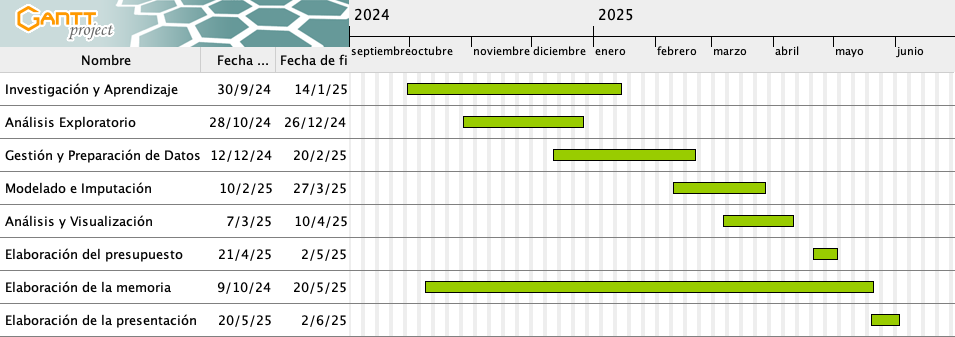
\includegraphics[width=0.9\textwidth]{images/planificacion.png} 
    \captionof{figure}{Diagrama de Gantt de la planificación inicial estimada para la realización del TFG.}
    \label{fig:gantt_planificacion}

    \vspace{1cm} 
    % Figura 2: Cronograma Real
    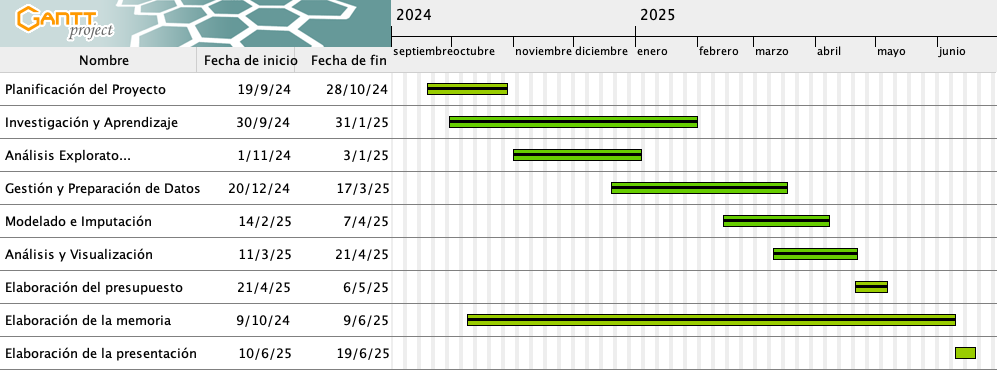
\includegraphics[width=0.9\textwidth]{images/cronograma.png}
    \captionof{figure}{Diagrama de Gantt del progreso real durante la realización del TFG.}
    \label{fig:gantt_cronograma_real}

\end{figure}

La comparación entre ambos cronogramas evidencia que el desarrollo real del proyecto sufrió una desviación con respecto a la planificación inicial. Este retraso se debió principalmente a los siguientes factores:
\begin{itemize}
    \item \textbf{Profundización en el Estado del Arte:} La revisión bibliográfica y el estudio de trabajos previos requirieron más tiempo del previsto para establecer una base teórica robusta y contextualizar adecuadamente el proyecto.
    \begin{itemize}
    \item \textbf{Complejidad de la Arquitectura Transformer:} Comprender en detalle los mecanismos de atención y la implementación de los modelos Transformer supuso una inversión de tiempo considerable, fundamental para su correcta aplicación.
    \end{itemize}
    \item \textbf{Curva de Aprendizaje de Bibliotecas:} La familiarización y el manejo eficiente de las bibliotecas de Python utilizadas (e.g., PyPOTS basada en PyTorch, Pandas, Numpy para manipulación de datos y Seaborn para visualización) implicaron un periodo de adaptación necesario para la implementación práctica.
\end{itemize}


\section{Metodología Utilizada}

La metodología adoptada en este Trabajo de Fin de Grado se enmarca en la tipología de \textbf{TFG de investigación}, dado que su propósito es generar conocimiento y validar una hipótesis mediante un proceso sistemático. Dicha investigación se sustenta en una \textbf{fundamentación matemática}. Este rigor teórico se complementa con una \textbf{revisión sistemática} del estado del arte, que garantiza una comprensión de las técnicas de imputación existentes y posiciona las contribuciones del trabajo.

En el aspecto práctico, la construcción del paquete de software se llevó a cabo siguiendo una \textbf{metodología ágil}, en particular el marco de trabajo \textbf{Scrum}, lo que permitió un desarrollo iterativo y adaptable. El proceso general de investigación siguió las etapas del \textbf{método científico} , desde la formulación del problema y la hipótesis, hasta el diseño y ejecución de experimentos empíricos con evaluación de resultados. Este enfoque integrado de investigación fundamental y desarrollo práctico busca ofrecer una solución validada al desafío de la imputación de datos en series temporales multivariantes.

% --- Texto Presupuesto y Anexo B ---
\section{Análisis del Presupuesto del Proyecto}

El presupuesto presentado a continuación se basa en la contabilización precisa de las horas dedicadas a cada tarea del TFG, registradas sistemáticamente con Timewarrior a lo largo de todo el desarrollo. Para la valoración económica, se ha aplicado la tarifa de 20 euros/hora. \citep{MemoriaTFG}

Para facilitar la comprensión y el análisis del presupuesto, el trabajo registrado se ha clasificado en tres categorías principales, siguiendo una estructura habitual:
\begin{itemize}
    \item \textbf{Parte teórica:} Recoge las tareas relacionadas con el análisis conceptual, el estudio del estado del arte y la fundamentación teórica del proyecto. Corresponde a la categoría agrupada \textit{Investigación y Aprendizaje}.
    \item \textbf{Parte práctica:} Reúne las actividades directamente vinculadas con la implementación, programación, experimentación, análisis de datos y validación. Engloba las categorías de \textit{Pipeline y Datos}, \textit{Modelado y Entrenamiento}, \textit{Imputación y Nulos}, \textit{Análisis y Visualización}, y \textit{Metodología y Estructura}.
    \item \textbf{Parte general:} Agrupa las labores transversales de gestión del proyecto, comunicación (reuniones con tutores, correos), documentación y elaboración de la memoria. Corresponde a la categoría \textit{Gestión y Comunicaciones}.
\end{itemize}
Además de los costes derivados de las horas de trabajo, se incluye el coste amortizado del equipamiento principal utilizado (Macbook Air M2), considerando una vida útil estimada de 7 años \footnote{\url{https://www.refurb.me/es/blog/cuanto-dura-un-macbook}}. El desglose detallado del presupuesto se presenta en el (Cuadro~\ref{tab:presupuesto_tfg_simplificado_v2}).

\section{Presupuesto Estimado}


\begin{table}[htbp]
    \scriptsize % Fuente pequeña para asegurar que quepa
    \centering
    \setlength{\tabcolsep}{4.5pt} % Ajustar el espaciado entre columnas
    \caption{Estimación Detallada del Coste de Desarrollo del Proyecto (\glsentryshort{tfg}) - Duración 9 Meses}
    \label{tab:presupuesto_tfg_simplificado_v2} % Nueva label para distinguir esta versión
    \begin{tabular}{l S[table-format=3.1] S[table-format=6.2] S[table-format=5.2] S[table-format=6.2]}
        \toprule
        \textbf{Concepto} & {\textbf{Horas}} & {\textbf{Coste Bruto \newline (Sueldo)}} & {\textbf{Coste SS \newline (Empresa)}} & {\textbf{Coste Total \newline Proyecto}} \\
         & {} & {(\textit{euros})} & {(\textit{euros})} & {(\textit{euros})} \\
        \midrule

        % --- COSTE DE PERSONAL (TODAS LAS TAREAS DE DESARROLLADOR A 20€/H) ---
        \multicolumn{5}{l}{\textbf{1. Coste de Personal}} \\
        \quad Gestión y Comunicaciones & 1.1 & 22.00 & 6.58 & 28.58 \\ % 1.1 * 20 = 22.00; 22.00 * 0.299 = 6.58; 22.00 + 6.58 = 28.58
        \quad Investigación y Aprendizaje & 223.9 & 4478.00 & 1339.42 & 5817.42 \\ % 223.9 * 20 = 4478.00; 4478.00 * 0.299 = 1339.42; 4478.00 + 1339.42 = 5817.42
        \quad Pipeline y Datos & 35.0 & 700.00 & 209.30 & 909.30 \\ % 35.0 * 20 = 700.00; 700.00 * 0.299 = 209.30; 700.00 + 209.30 = 909.30
        \quad Modelado y Entrenamiento & 32.6 & 652.00 & 194.95 & 846.95 \\ % 32.6 * 20 = 652.00; 652.00 * 0.299 = 194.95; 652.00 + 194.95 = 846.95
        \quad Imputación y Nulos & 185.3 & 3706.00 & 1108.09 & 4814.09 \\ % 185.3 * 20 = 3706.00; 3706.00 * 0.299 = 1108.09; 3706.00 + 1108.09 = 4814.09
        \quad Análisis y Visualización & 5.6 & 112.00 & 33.49 & 145.49 \\ % 5.6 * 20 = 112.00; 112.00 * 0.299 = 33.49; 112.00 + 33.49 = 145.49
        \quad Metodología y Estructura & 3.5 & 70.00 & 20.93 & 90.93 \\ % 3.5 * 20 = 70.00; 70.00 * 0.299 = 20.93; 70.00 + 20.93 = 90.93
        \quad Tutores (2 personas) & 72.0 & 2880.00 & 861.12 & 3741.12 \\ % 72.0 * 40 = 2880.00; 2880.00 * 0.299 = 861.12; 2880.00 + 861.12 = 3741.12
        \midrule
        \textbf{Subtotal Coste de Personal} & \textbf{559.0} & \textbf{12620.00} & \textbf{3773.88} & \textbf{16393.88} \\
        \midrule

        % --- COSTE DE MATERIAL (HARDWARE/SOFTWARE) ---
        \multicolumn{5}{l}{\textbf{2. Coste de Material (Hardware/Software)}} \\
        \quad Amortización Macbook Air M2 (9 meses de uso) & {} & {} & {} & 139.29 \\
        \midrule
        \textbf{Subtotal Coste de Material} & {} & {} & {} & \textbf{139.29} \\
        \midrule

        % --- COSTES INDIRECTOS ---
        \multicolumn{5}{l}{\textbf{3. Costes Indirectos (Estimación 9 meses)}} \\
        \quad Suministro Eléctrico & 9 \text{ meses} & {} & {} & 293.81 \\
        \quad Suministro de Agua & 9 \text{ meses} & {} & {} & 221.49 \\
        \quad Conexión a Internet & 9 \text{ meses} & {} & {} & 180.00 \\
        \midrule
        \textbf{Subtotal Costes Indirectos} & {} & {} & {} & \textbf{695.30} \\
        \midrule

        % --- COSTE TOTAL DEL PROYECTO ---
        \textbf{COSTE TOTAL ESTIMADO DEL PROYECTO} & {} & {} & {} & \textbf{17228.47} \\ % 16393.88 + 139.29 + 695.30 = 17228.47
        \bottomrule
    \end{tabular}
    \par\medskip
    \footnotesize
    \textit{Nota: El coste de personal se basa en las horas registradas, aplicando una tarifa bruta consolidada de 20 €/hora para todas las tareas de desarrollador. Para el rol de Tutor, la tarifa se ha fijado en 40 €/hora (basado en 2 horas/semana durante 9 meses). Los costes de Seguridad Social a cargo de la empresa se han calculado como un 29.9\% del coste bruto del sueldo. El Impuesto sobre la Renta de las Personas Físicas (IPRF) es una retención aplicada al sueldo bruto del trabajador (no un coste adicional para el proyecto). La amortización del equipo considera un uso de 9 meses para el proyecto sobre una vida útil de 7 años (coste original del equipo 1300€). Los costes indirectos son una estimación mensual prorrateada para la duración supuesta del proyecto (9 meses).}
\end{table}

\clearpage % Opcional

% --- FIN CÓDIGO PARA anexos.tex ---